\chapter{DESIGN AND IMPLEMENTATION}
\label{chap:desainandimplementation}

% Ubah bagian-bagian berikut dengan isi dari desain dan implementasi

This chapter describes the design and implementation of the system that has been created.
As seen in Figure \ref{fig:block-diagram}, it starts with making a new dataset. Then, training pose estimation models for humanoid robot with that new dataset.
After that, we search the best model for both human and humanoid robot. Lastly, we make a main program that compares the suitability between humanoid robot pose and human pose.

\begin{figure}[ht]
  \centering
  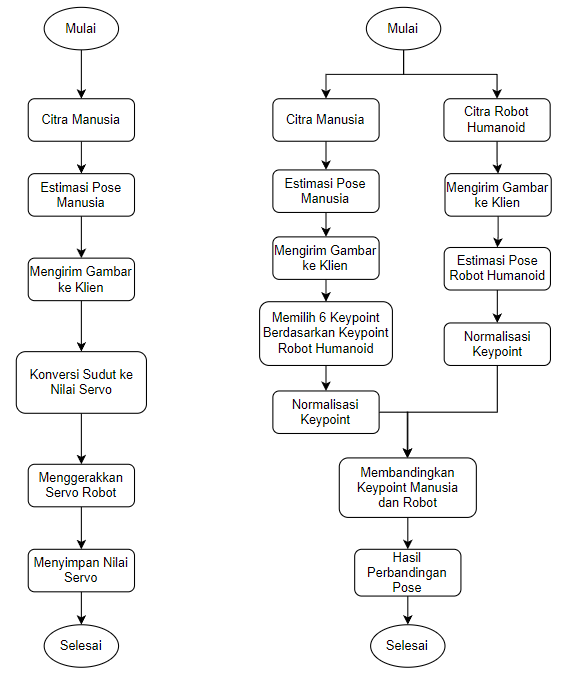
\includegraphics[scale=1.1]{gambar/diagram-block.png}
  \caption{Block Diagram of Workflow.}
  \label{fig:block-diagram}
\end{figure}

\section{Make New Dataset}
\label{sec:makenewdataset}

This new dataset is a merge of KimbRo's Humanoid Robot Pose dataset and Ichiro's dataset. NimbRo's dataset contains both single and multiple robots to
simulate RoboCup's real conditions. They also gathered from RoboCup Humanoid League YouTube videos, their own internal videos, and ROS bags. 
Overall, their dataset has over 1.5k images that come from 23 videos with around 2.3k robot instances. These images include teen and adult-sized robots and contain more than ten different robot types \parencite{amini2021}.
However, the robots in Ichiro's dataset are only kid-sized and come in single or maximum two-robot configurations. The images in our dataset come from videos that are taken in our lab. 
Then we split up those videos into multiple images and we pick not blurred videos.
Before merging, we need to fix NimbRo's dataset format first. This is because after we visualized some of their data, we found that the bounding boxes in \emph{annotations} part were misplaced (the width and height were swapped).
After we refine their dataset format and merge them with our dataset, the newly created dataset has approximately 2.1k images.
About 20 percent of the dataset was used for scoring and validating.

When it comes to annotation tools, there are a lot of choices out there including offline and online tools. We have tried some of them like Dataloop, V7labs, or Supervisely which is recommended by NimbRo.
However, when we tried to export the dataset into COCO format, it failed (e.g. can not import it or it can be imported but the JSON result in the annotation section is none). So, we decided to use a coco-annotator,
a web-based image annotation tool designed for versatility and efficiently labeling images to create training data. Regarding the number of keypoints in each robot, we followed NimbRo's dataset.
There are six keypoints including head, trunk, hands, and feet. We stick to that idea because we want to try the model's performance and inference time with fewer keypoints first and if we are confident enough, we will increase the number of keypoints later.


\section{Training Pose Estimation Model for Humanoid Robot}
\label{sec:trainingrobot}

All of the training processes in this study were primarily conducted on a DGX-A100 server computer and written in the Python programing language. The specific configuration explains in Table \ref{tb:dgxa100}.
From this base specification, we are allocated a Jupiter notebook container with
python and many libraries preinstalled with following allocated resources explained in Table \ref{tb:allocatedcontainer}.

\begin{longtable}{|c|c|}
  \caption{DGX-A100 Specification.}
  \label{tb:dgxa100}\\
  \hline
  CPU     & Dual AMD Rome 7742, 128 cores total @ 2.25 GHz \\
  \hline
  GPU     & 8 x NVIDIA A100 80 GB Tensor Core GPUs  \\
  \hline
  RAM     & 2 TB \\
  \hline
  Storage & 30 TB (8 x 3.84 TB) U.2 NVMe drives \\
  \hline
\end{longtable}

\begin{longtable}{|c|c|}
  \caption{Allocated container specification.}
  \label{tb:allocatedcontainer}\\
  \hline
  GPU     & 1/4 NVIDIA A100 GPU \\
  \hline
  GPU RAM & 20 GB  \\
  \hline
  CPU RAM & 8 GB \\
  \hline
  Storage & 100 GB  \\
  \hline
\end{longtable}

\subsection{NimbRo's Model}
\label{subsec:trainingnimbromodel}

The hyperparameters that are used to train NimbRo's model followed the description in their paper.
This model is trained using the AdamW optimizer with a learning rate of 10\textsuperscript{-4} ,
batch size 16, and weight decay of 10\textsuperscript{-4} for the total 200 epochs.
Note that the encoder is initialized by pre-trained ResNet weights on ImageNet.
We also use data augmentation that includes random horizontal flip, random
rotation, random scaling, and random translation during training \parencite{amini2021}.

The main program for training is already made by them named \emph{main.py} using PyTorch framework, we just need to run it on Jupyter Notebook file or Terminal and adjust the arguments for our needs
as seen in Command \ref{lst:trainingnimbro}. The value of argument \emph{config} is a file where we store all the hyperparameters, File \ref{lst:confignimbro} is one of the example.
Second argument is a directory path where we save training result and last argument is a directory path where the dataset takes place.

\begin{lstlisting}[
  language={},
  caption={Training NimbRo command.},
  label={lst:trainingnimbro}
]
python src/main.py --config experiments/train_merge_2.yaml --output_dir ichiro_nimbro_merge --dataset_path dataset/hrp/
\end{lstlisting}

\lstinputlisting[
  language={},
  caption={Example YAML file config for NimbRo's Training.},
  label={lst:confignimbro}
]{files/train_nimbro.yaml}

\subsection{YOLO-pose}
\label{subsec:trainingyolopose}

Before we jumped into training process, we must change format of our newly dataset from COCO to YOLO. Differ from COCO format, YOLO format give keypoint confidence or visibility flag 2 for either visible or occluded keypoint
and if it is outside the field of view, the value is set to zero. However, COCO format defined visibility flag as v=0: not labeled,  v=1: labeled but not visible, and v=2: labeled and visible. So, we change the definition of
v=1 and v=2 become just v=2 in YOLO format and keep v=0.
Beside keypoint format differences, bounding-box format between them is also different. COCO defines a bounding-box as follow: x (top left), y (top left), width, and height. On the other hand,
bounding-box format in YOLO is: x (center), y (center), width, and height also all of them need to be normalized. Thus, we need to add 1/2 width to x, 1/2 height to y, and normalize them.
All of that processes can be seen in Code \ref{lst:changecocotoyolo}. 

\lstinputlisting[
  language=Python,
  caption={Change COCO to YOLO format program.},
  label={lst:changecocotoyolo}
]{program/coco-to-yolo.py}

The hyperparameters to train YOLO-pose followed the description in their GitHub named \emph{hyp.pose.yaml}.
We use SGD optimizer with a cosine scheduler. The base learning rate is set to 10\textsuperscript{-2}, batch size 16,
and weight decay of 5\textsuperscript{-4} for total 150 epochs. There are also data augmentation like random scale ([0.5, 1.5]),
random translation [-10, 10], random flip with probability 0.5, mosaic augmentation with probability 1, and various color augmentations.
It is the same with Section \ref{subsec:trainingnimbromodel}, actually, the main program for training has been provided using PyTorch framework too, but the program is intended for humans with 17 keypoints.
If we run it directly with our dataset with 6 keypoints, an error will be raised. Therefore, a little bit of code needs to be changed to make the training process can be run.
After that, we can run Command \ref{lst:trainingyolo}. We will not go into all the arguments, only some of them. 
A file containing the dataset path, number of keypoint, and class name is on the first argument. The second argument explains the full network architecture of YOLO-pose and 
argument \emph{hyp} is a file contains all the hyperparameters that are used.

\begin{lstlisting}[
  language={},
  caption={Training YOLO-pose command.},
  label={lst:trainingyolo}
]
python train.py --data data/robot_kpts.yaml --cfg cfg/yolov7-w6-robot-pose.yaml --weights weights/yolov7-w6-pose.pt --batch-size 8 --kpt-label --device 0 --name yolov7-pose-merge --hyp data/hyp.pose.yaml --epochs 150
\end{lstlisting}

\subsection{Keypoint RCNN}
\label{subsec:trainingrcnn}

The Keypoint RCNN training is done on Jupyter Notebook directly using the PyTorch framework as well.
Before starting the training process, we also need to convert the dataset format first.
Actually, this format is almost the same as the YOLO format (each image has its own label), but the difference lies in the bounding box.
Where the format of the bounding-box is the top left point and the bottom right point. We can do that by running Code \ref{lst:changecocotorcnn}.

\lstinputlisting[
  language=Python,
  caption={Change COCO to RCNN format program.},
  label={lst:changecocotorcnn}
]{program/coco-to-rcnn.py}

The training process starts with loading our dataset and specifying the augmentation technique we are using. We use \emph{albumentations} library for augmenting our dataset.
At first, we apply random rotation, brightness, and contrast. Nevertheless, the model seems to become underfitting, so we try just random brightness and contrast as seen in Code \ref{lst:augmentationrcnn}. 
Fortunately, the result seems pretty good after that.

\lstinputlisting[
  language=Python,
  caption={Augmentation technique used in RCNN Training.},
  label={lst:augmentationrcnn}
]{program/rcnn-augmentation.py}

Code snippet \ref{lst:rcnnmodeldefinition} is a function that returns the Keypoint RCNN model.
When calling the function, we can fill the first argument with value 6
and leave the second argument blank. After the training process is complete, we can call the function again and fill in the second argument with the path of the resulting model for keypoint detection process.
By default, the AnchorGenerator class in PyTorch has 3 different sizes (128, 256, 512) and 3 different aspect ratios (0.5, 1.0, 2.0).
We have extended those parameters, AnchorGenerator to (32, 64, 128, 256, 512) and aspect ratios to (0.25, 0.5, 0.75, 1.0, 2.0, 3.0, 4.0).
Note that, \emph{num classes} argument is set to two because the first class is background and object is the second class.
In this training, we use SGD optimizer with learning rate 10\textsuperscript{-3}, batch size 3, and weight decay of 5\textsuperscript{-4} for 50 epochs.

\lstinputlisting[
  language=Python,
  caption={Keypoint RCNN model definition in PyTorch.},
  label={lst:rcnnmodeldefinition}
]{program/rcnn-model.py}


\section{Finding the Best Model for Humanoid Robot Pose Estimation}
\label{sec:findingbestmodelhumanoidrobot}

We compare the three models on Section \ref{sec:trainingrobot} based on \emph{mAP} (mean Average Precision), \emph{mAR} (mean Average Recall),
real detection result, and inference time on devices with limited computing capabilities (e.g. NUC i5).
The comparison table of \emph{mAP}, \emph{mAR}, and real detection result of those models are in Chapter \ref{chap:resultsandiscussion}. In this section we just talk about the time inference.
To know the time that it takes for the model to do the detection, we just need to subtract the time before and after the model does keypoint detection like Code \ref{lst:timedifference}.

\lstinputlisting[
  language=Python,
  caption={Time difference program.},
  label={lst:timedifference}
]{program/time-difference.py}

We attempt converting our models from PyTorch Model to OpenVINO in order to speed up the time inference. Before that, we convert it to ONNX first like Figure \ref{fig:pytorch-to-openvino}.
The steps for converting PyTorch Model to ONNX can be seen in Code \ref{lst:convertpytorchtoonnx}. At first, we must ensure that the model is in inference mode by calling \emph{eval} function.
Next, we create that dummy input variable. The call to \emph{torch.onnx.export} function runs the model once to trace its execution and then exports the traced model to the specified file.
The resulting \emph{model-name.onnx} file contains a binary protocol buffer which contains both the network structure and parameters of the model exported.
After that, we use Model Optimizer to convert the ONNX model to OpenVINO IR with FP16 precision. To install Model Optimizer in Python is pretty simple, just run
\emph{pip install openvino-dev} in Terminal and to verify the package is properly installed, we run the command \emph{mo -h}. We will see the help message for Model Optimizer if installation finished successfully.
After we run Command \ref{lst:convertonnxtoopenvino}, in directory named model, there are three files with \emph{bin}, \emph{mapping}, and \emph{xml} extension.
If we want to run OpenVINO IR Model in OpenVINO Runtime, look Code \ref{lst:runopenvino}. Note that, the model path must contain three files earlier.

\begin{figure}[ht]
  \centering
  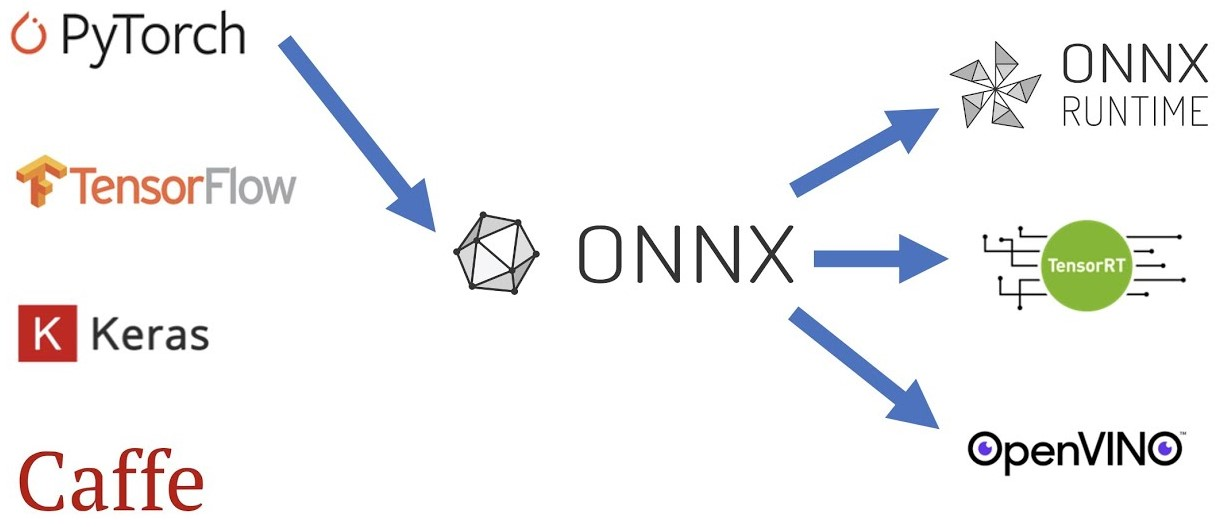
\includegraphics[scale=0.45]{gambar/pytorch-onnx-openvino.jpg}
  \caption{Flow of converting PyTorch Model to OpenVINO.}
  \label{fig:pytorch-to-openvino}
\end{figure}

\lstinputlisting[
  language=Python,
  caption={Convert from PyTorch Model to ONNX program.},
  label={lst:convertpytorchtoonnx}
]{program/convert_pytorch-to-onnx.py}

\begin{lstlisting}[
  language={},
  caption={Convert ONNX to OpenVINO command.},
  label={lst:convertonnxtoopenvino}
]
mo --input_model 'model-name.onnx' --compress_to_fp16 --output_dir 'model'
\end{lstlisting}

\lstinputlisting[
  language=Python,
  caption={Run OpenVINO IR Model in OpenVINO Runtime.},
  label={lst:runopenvino}
]{program/load-openvino.py}


\section{Finding the Best Model for Human Pose Estimation}
\label{sec:findingbestmodelhumanrobot}


\section{Comparing the Suitability Between Humanoid Robot Pose and Human Pose}
\label{sec:comparingsuitability}

Before comparing the pose between a human and a humanoid robot, we need to reduce the human keypoint to the same as the robot's keypoint.
Based on the results after testing, we chose Mediapipe for human and Keypoint RCNN for robot. Mediapipe provides 33 landmark keypoints for human and Keypoint RCNN only provides 6 keypoints.
Therefore, we need to reduce the human keypoint to 6 as shown in Code \ref{lst:reducehumankeypoints}.
The name of the keypoints in the code corresponds to the name of the keypoints in the robot. First, we get all 33 keypoints in row 16. Then calculate the keypoint we want, such as the head keypoint which is located between the right and left eyes.
The keypoint for the hands and feet is simply to select the wrists and ankles in Mediapipe(lines 22-28), where landmark[15] and landmark[16] are wrists, landmark[27] and landmark[28] are ankles. Lastly, the trunk keypoint is located between the shoulder and hip keypoint (lines 31-34).

\lstinputlisting[
  language=Python,
  caption={Reduce human keypoints program.},
  label={lst:reducehumankeypoints}
]{program/reduce-human-keypoints.py}

The next step is defining similarity. When we think about the problem, we see that there are many uncertainties to be addressed. For example, human and humanoid robot can differ in height, body shape, and location within an image: one subject (human or robot) may have been nearby the camera,
while another may have been in the distance. In order to get an accurate outcome, each of these issues must be resolved.
After reducing the keypoints, the model output for both human and robot is the coordinates of 6 keypoints. This information can be used to create a new bounding box that tightly covers the person in the picture. This solves the problem of the subject appearing in different parts of the picture.
We further normalized the resulting keypoints coordinates by performing L2 normalization in order to transform it into a unit vector as shown in Figure \ref{fig:transforming-into-unit-vector}. This means we are ignoring the size of the picture, but keeping in account the direction of the vector, created by the pose inside of that image.
The two steps described before can be thought of visually as shown in Figure \ref{fig:steps-to-normalize}.

\begin{figure}[ht]
  \centering
  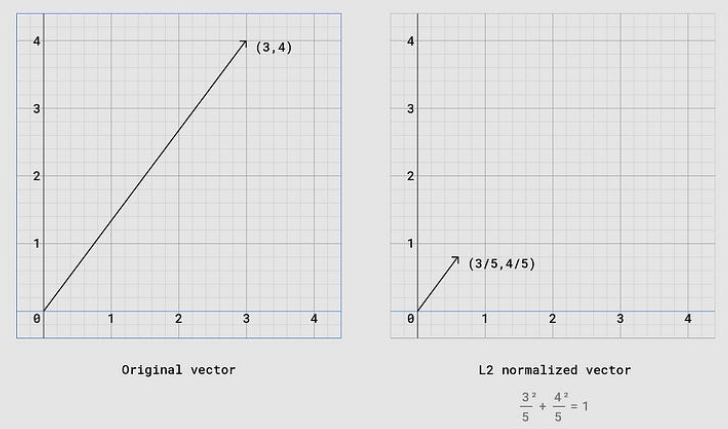
\includegraphics[scale=0.9]{gambar/transform-to-unit-vector.png}
  \caption{Transforming into Unit Vector.}
  \label{fig:transforming-into-unit-vector}
\end{figure}

\begin{figure}[ht]
  \centering
  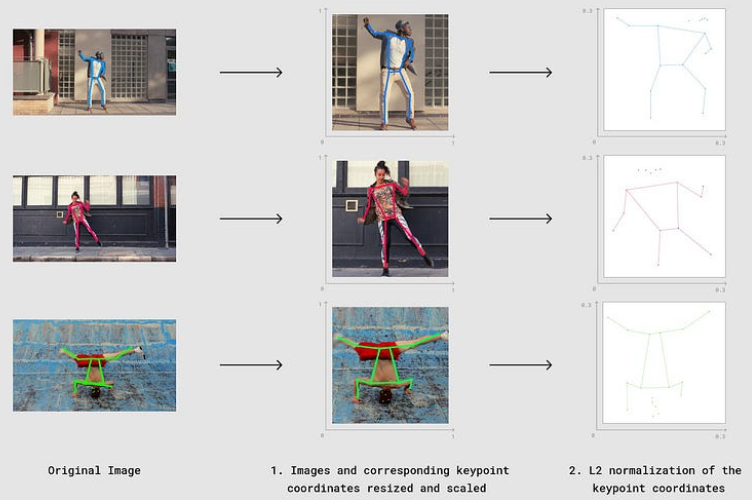
\includegraphics[scale=0.9]{gambar/two-steps.png}
  \caption{Steps Taken to Normalize Data.}
  \label{fig:steps-to-normalize}
\end{figure}

Now that we have standardized the pose vectors, it is time to choose a similarity measure. We chose cosine similarity for this particular instance, mainly because we are working with vectors and performing a few calculations detailed below to arrive at a Euclidean distance that can be interpreted as a cosine distance. The formula shown in Equation \ref{eq:euclideandistance}.
In that formula, Fxy and Gxy are two pose vectors to be compared after L2 normalization. Moreover, Fxy and Gxy contain only x and y positions for each of the 6 keypoints, it does not include confidence scores.

\begin{equation}
  \label{eq:euclideandistance}
  \sum \mathbf{F} = 0\; \Leftrightarrow\; \frac{\mathrm{d} \mathbf{v} }{\mathrm{d}t} = 0.
\end{equation}

\section{Making Main Program}
\label{sec:makingmainprogram}